\documentclass[twoside,12pt]{wipb}

\katedra{Nazwa katedry}
\typpracy{in�ynierska}
%typpracy{magisterska}
\temat{Edytor modeli 3D opartych\newline o woksele}
\autor{Pawe� Aleksiejuk}
\promotor{dr in�. �ukasz Gadomer}
\indeks{105527}
\studia{stacjonarne}
\rokakademicki{2021/2022}
\profil{studia I stopnia}
\kierunekstudiow{Informatyka}
\specjalnosc{In�ynieria Oprogramowania}
\zakres{1. Przegl�d podobnych rozwi�za� dost�pnych na rynku.\newline 2. Zdefiniowanie wymaga� stawianych wobec rozwi�zania.\newline 3. Opracowanie prostego silnika 3D.\newline 4. Stworzenie narz�dzia do edycji modelu 3D\newline 5. Testowanie stworzonego rozwi�zania.}

\hypersetup{
pdfauthor={Pawe� Aleksiejuk},
pdftitle={Praca in�ynierska},
pdfsubject={Edytor modeli 3D opartych o woksele},
pdfkeywords={praca in�ynierska jakie� inne s�owa kluczowe},
pdfpagemode=UseNone,
linkcolor=black,
citecolor=black,
urlcolor=black
} 

\setlength{\epigraphwidth}{1\textwidth}
\setlength{\parskip}{0.2em}
\usepackage{enumitem}
\usepackage{listings}

\begin{document}
\maketitle

\cleardoublepage
\chapter*{\centering{\vspace{1in}Summary}}
\addcontentsline{toc}{chapter}{Streszczenie}
 
\epigraphhead[40]{
Subject of diploma thesis

3D model editor based on voxels}

Graphics in modern usage is mainly associated with computer representation of data.
We most commonly distinguish between two types of graphics: 2D (two-dimensional)
and 3D (three-dimensional). 2D graphics involve presenting a visual output based on a
two-dimensional object, while 3D graphics, involve a three-dimensional object.

A voxel is a representation of a point in a three-dimensional space. The name voxel originated from a combination of the words, volume and element and is similar to a picture and an element in the case of a pixel.

Interested in these topics, the author decided to trace the creation of 3D graphics back
to the model editor, creating one from scratch as part of this work. This editor is intended to allow the user to create a voxel-based 3D model using built-in editing mechanisms.

The motivation for writing this thesis was to create a simple functional 3D engine,
along with tools for creating models using this engine. Later on, I plan to extend this project by creating a fully functional 3D game.
\clearpage
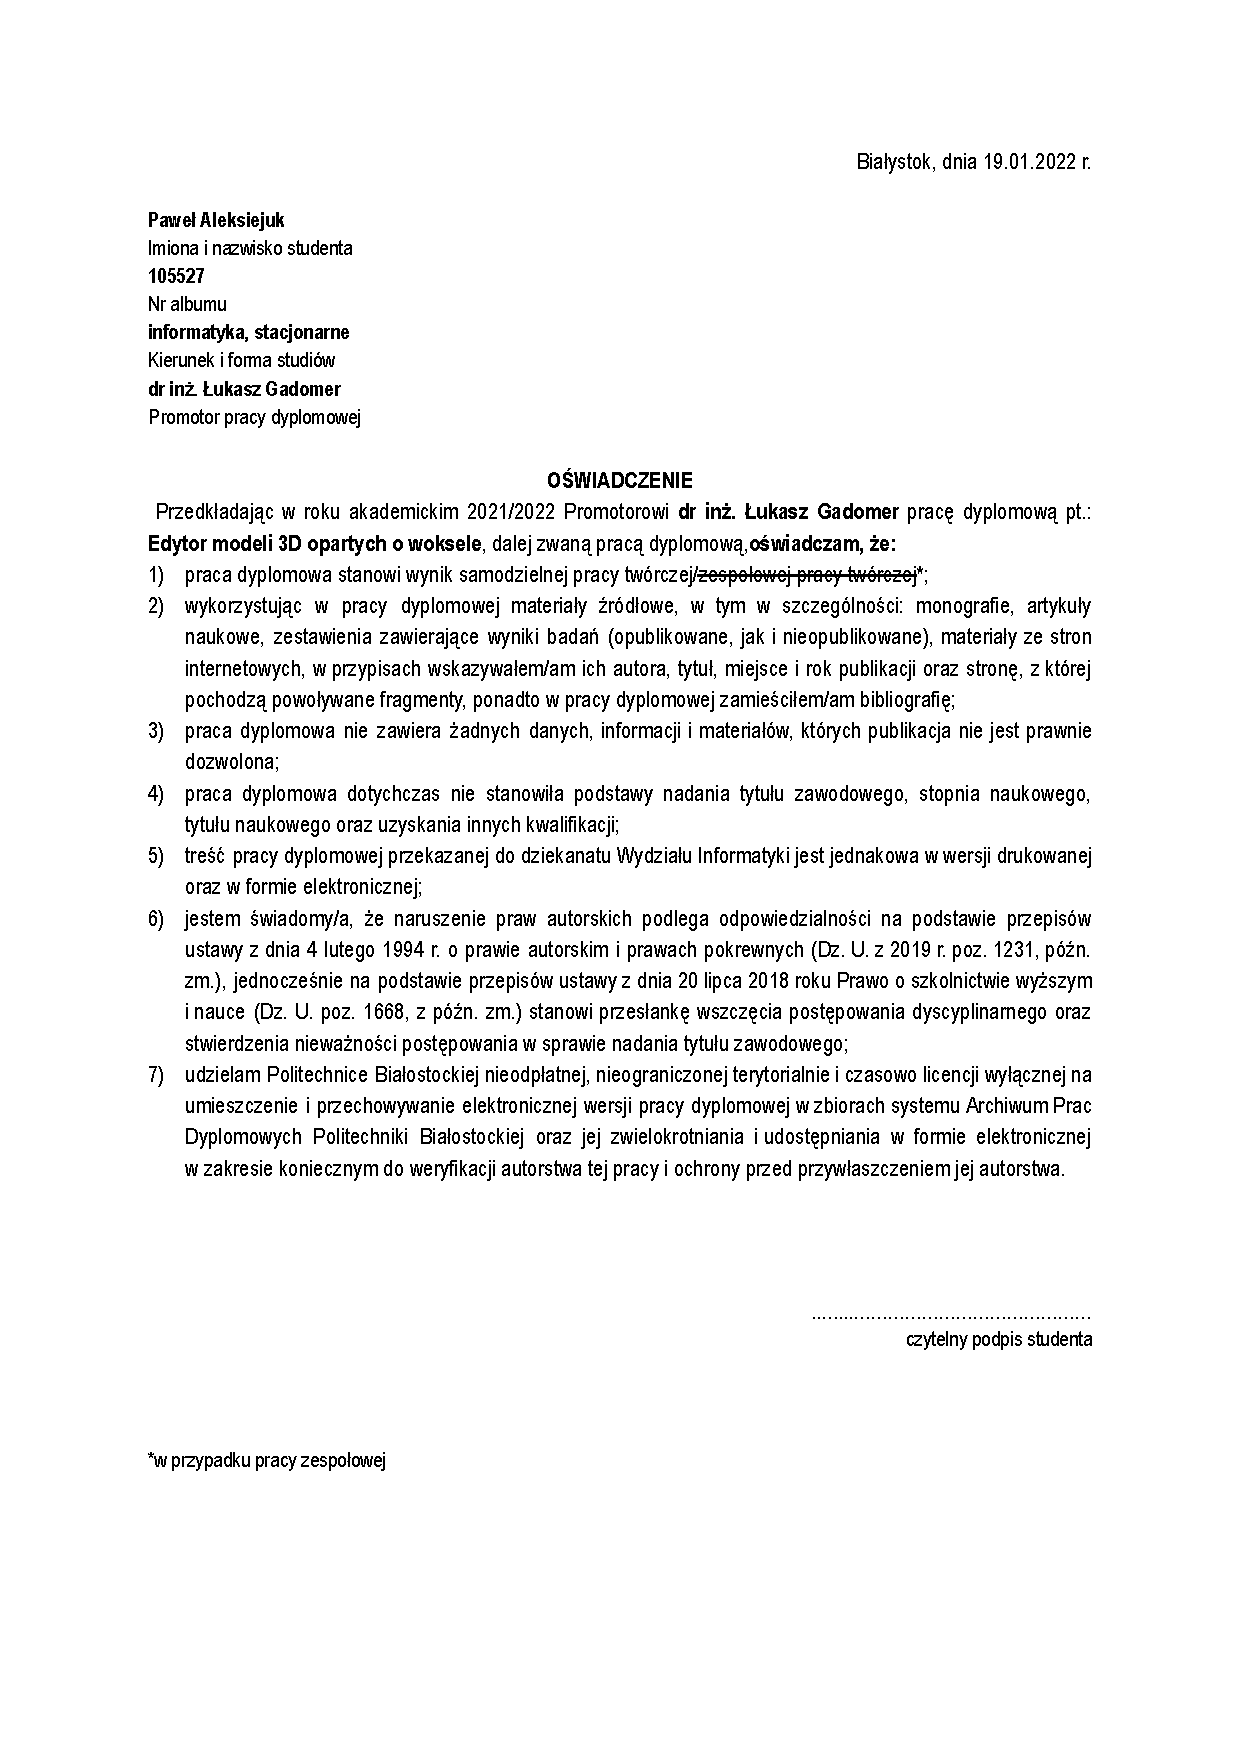
\includepdf[pages={1}]{grafika/oswiadczenie-o-samodzielnosci.docx.pdf}




%\biblioteka{}

\pagestyle{plain}

\setcounter{tocdepth}{1}
\tableofcontents

\chapter*{Wst�p}
\addcontentsline{toc}{chapter}{Wst�p}

Grafika we wsp�czesnym u�yciu kojarzy si� g��wnie z komputerowym przedstawieniem danych. Dane te tworz� medium wizualne, kt�re mog� by� wy�wietlane mi�dzy innymi na ekranach naszych monitor�w komputerowych. Najcz�ciej rozr�niamy dwie rodzaje grafik: 2D (ang. \textit{two-dimensional}) i 3D (ang. \textit{three-dimensional}). Grafika 2D polega na przedstawieniu medium wizualnego opartego na obiekcie o dw�ch wymiarach, za� grafika 3D, analogicznie na obiekcie o trzech wymiarach.


Wokselem (ang. \textit{voxel}) \cite{voxels_definition} nazywamy przedstawienie punktu w tr�jwymiarze. Nazwa woksel jest po��czeniem angielskich s��w \textit{volume} oraz \textit{element} i jest to analogiczne po��czenie do \textit{picture} i \textit{element} w przypadku piksela (ang. \textit{pixel}). Najcz�stszym sposobem 


Zainteresowany tymi tematami, autor postanowi� prze�ledzi� drog� tworzenia grafiki 3D od strony edytora modeli, tworz�c go od postaw w ramach tej pracy. Edytor ten ma pozwoli� u�ytkownikowi na kreacj� modelu 3D opartego na wokselach, wykorzystuj�c wbudowane mechanizmy edycji.


Motywacj� do napisania tej pracy by�o ch�� stworzenia prostego funkcjonalnego silnika graficznego wraz z narz�dziem do tworzenia modeli obs�ugiwanych przez ten silnik. W p�niejszym czasie, planuj� rozszerzy� ten projekt, tworz�c w pe�ni funkcjonaln� gr� 3D. 


Zakres pracy obejmowa�: 
\begin{itemize}
\item Przegl�d podobnych rozwi�za� dost�pnych na rynku.
\item Zdefiniowanie wymaga� stawianych wobec rozwi�zania.
\item Opracowanie prostego silnika 3D.
\item Stworzenie narz�dzia do edycji modelu 3D.
\item Testowanie stworzonego rozwi�zania.
\end{itemize}



Rozdzia� 1 przedstawia 5 istniej�cych ju� na rynku edytor�w graficznych opartych o woksele, w celu zaznajomienia si� z podstawowymi funkcjonalno�ciami postawionymi przez ich autor�w. 
 
Rozdzia� 2 skupia si� na przedstawieniu dog��bnie projektu systemu, w celu zapoznania si� z wymaganiami wobec aplikacji, jak i z wizj� systemu w formie graficznej.

Rozdzia� 3 opisuje zastosowane technologie i rozwi�zania, t�umacz�c logik� i motywacj� za wyborem ka�dych z nich. 

Rozdzia� 4 opisuje realizacje aplikacji. Zawiera w sobie informacje na temat technologii, �rodowiska programistycznego i implementacji.
\chapter{Przegl�d istniej�cych rozwi�za�}

Z uwagi na specjalistyczne zastosowanie stworzonego edytora graficznego, a mianowicie tworzenie specjalnych obiekt�w obs�ugiwanych przez wbudowany silnik graficzny, istniej�ce rozwi�zania w g��wnej mierze maj� s�u�y� jako wykaz podstawowych, jak i dodatkowych funkcjonalno�ci do mo�liwej implementacji w ostatecznym rozwi�zaniu.

\section{MagicaVoxel}

MagicaVoxel \cite{magicavoxel_page} jest najpopularniejszym darmowym desktopowym edytorem wokseli dost�pnym aktualnie na rynku. Stworzony i na bie��co aktualizowany przez u�ytkownika o pseudonimie @ephtracy pozwala na nie tylko tworzenie modeli, ale te� zdj�� do p�niejszego udost�pniania. Taka funkcjonalno�� pozwala na przetestowanie modelu w r�nych warunkach, kt�re s� edytowalne poprzez parametry w wewn�trznym silniku renderuj�cym. Interfejs  rozwi�zania zosta� przedstawiony na rysunku \ref{rys1.1-magicavoxel}

\begin{figure}[htb]
\centering
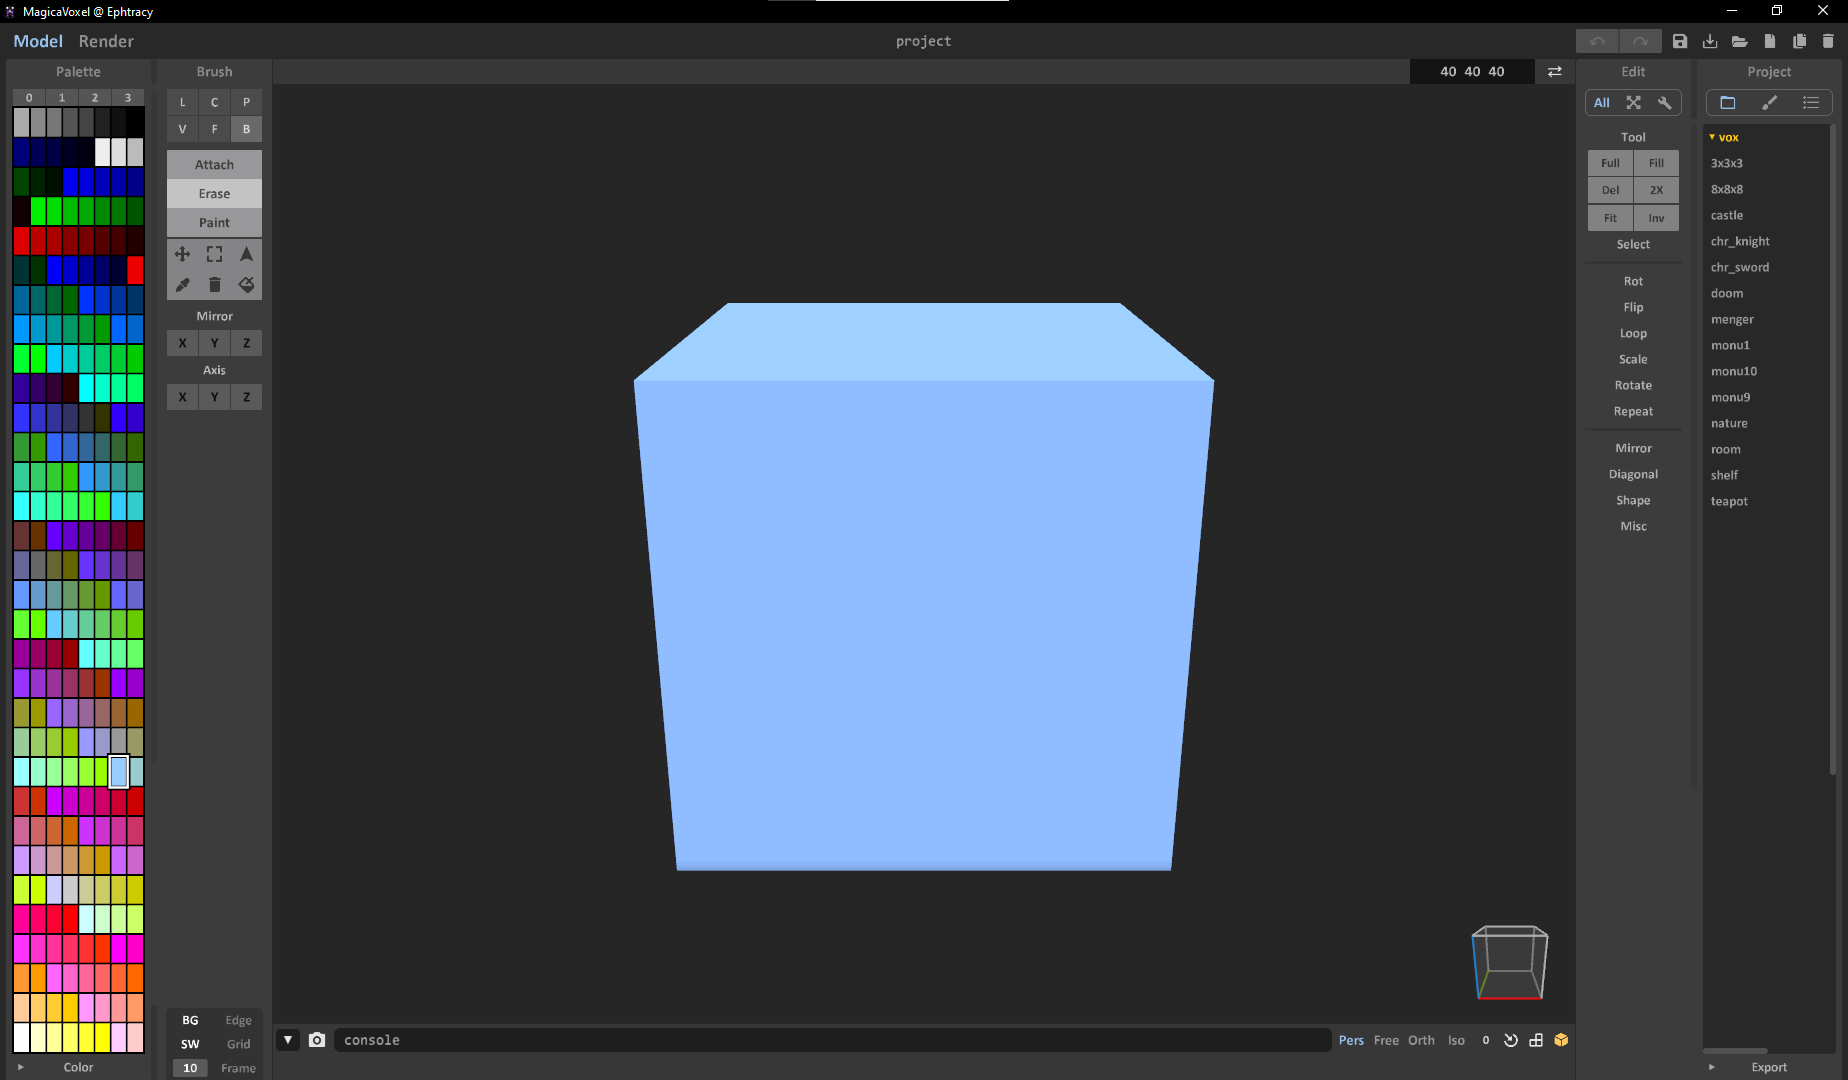
\includegraphics[width=0.9\textwidth, keepaspectratio]{grafika/magicavoxel.png}
\caption[Ekran startowy programu MagicaVoxel (Windows)]{Ekran startowy programu MagicaVoxel (Windows), �r�d�o: \cite{magicavoxel_page}}
\label{rys1.1-magicavoxel}
\end{figure}

G��wne atuty oprogramowania wed�ug producenta:
\begin{itemize}
\item Zaawansowany wewn�trzny silnik renderuj�cy. 
\item Ca�kowicie darmowe oprogramowanie, nawet w przypadku u�ycia komercyjnego.
\end{itemize}

MagicaVoxel jest dost�pny za darmo na platformach Windows i macOS.

\section{Mega Voxels Play}

Mega Voxels Play \cite{mega_voxels_play_page} to darmowy mobilny edytor stworzony przez Go Real Games. Tak jak wi�kszo�� edytor�w wokselowych, pozwala na podstawowe operacje takie jak dodawanie, usuwanie i malowanie. Aplikacja posiada wbudowany sklep, kt�ry pozwala na pobranie gotowych modeli, w celu p�niejszego wykorzystania. Interfejs  rozwi�zania zosta� przedstawiony na rysunku \ref{rys1.2-mega-voxels-play}

\begin{figure}[htb]
\centering
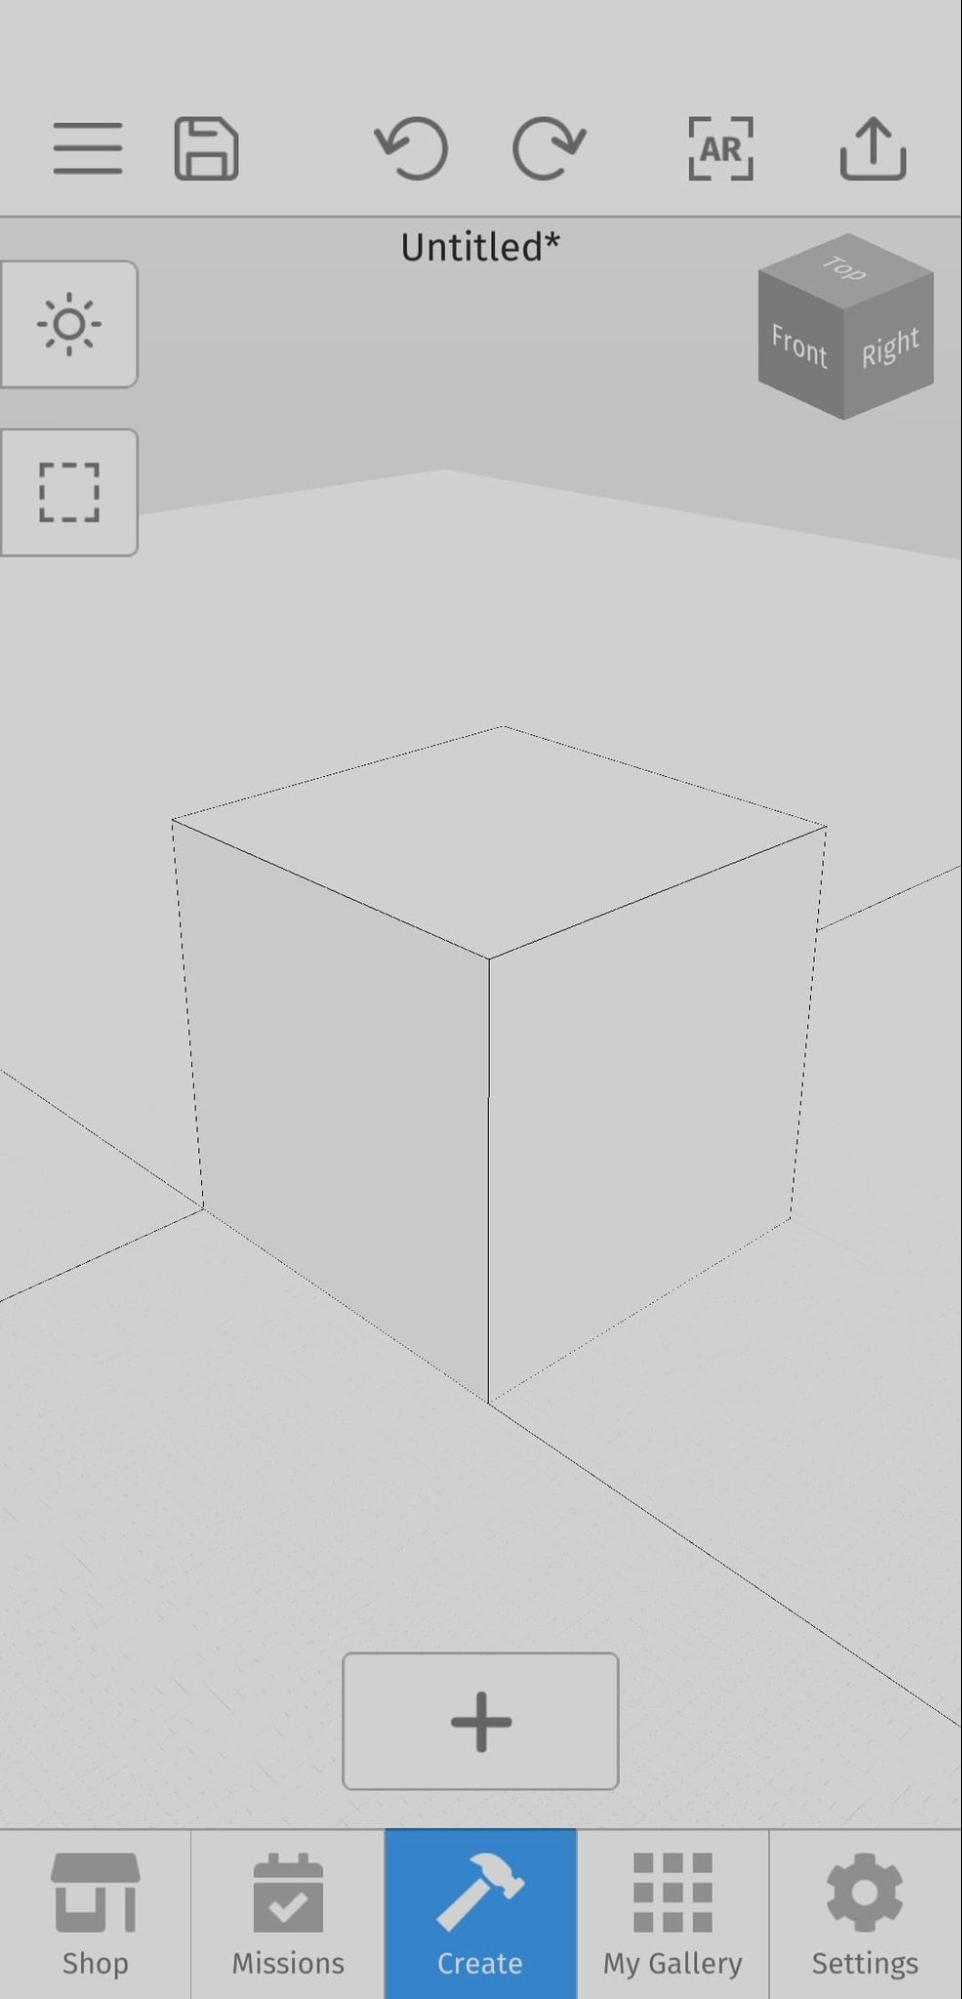
\includegraphics[width=0.8\textwidth, height=0.4\textheight, keepaspectratio]{grafika/mega-voxels-play.png}
\caption[Ekran startowy programu Mega Voxels Play (Android)]{Ekran startowy programu Mega Voxels Play (Android), �r�d�o: \cite{mega_voxels_play_page}}
\label{rys1.2-mega-voxels-play}
\end{figure}

G��wne atuty oprogramowania wed�ug producenta:
\begin{itemize}
\item Du�a ilo�� bazowych modeli do pobrania.
\item Prosto�� w obs�udze.
\item Wsparcie dla AR (Rozszerzonej rzeczywisto�ci).
\item R�ne efekty przetwarzania ko�cowego.
\end{itemize}

Mega Voxels Play jest dost�pny za darmo na platformach mobilnych (Android i iOS).

\section{Qubicle}

Qubicle \cite{qubicle_page} jest zaawansowanym desktopowym narz�dziem stworzonym przez Minddesk, przeznaczonym do tworzenia wokselowych modeli. Z por�wnaniem do poprzednik�w, aplikacja nie posiada limitu wielko�ci modeli, co pozwala u�ytkownikom na swobodne tworzenie wielkich modeli, jak i ca�ych teren�w. Dodatkowo opr�cz standardowego w edytorach formatu .obj (Wavefront File), wspierane s� te� takie formaty jak .fbx (Autodesk), .dae (Collada). Interfejs  rozwi�zania zosta� przedstawiony na rysunku \ref{rys1.3-qubicle}

\begin{figure}[htb]
\centering
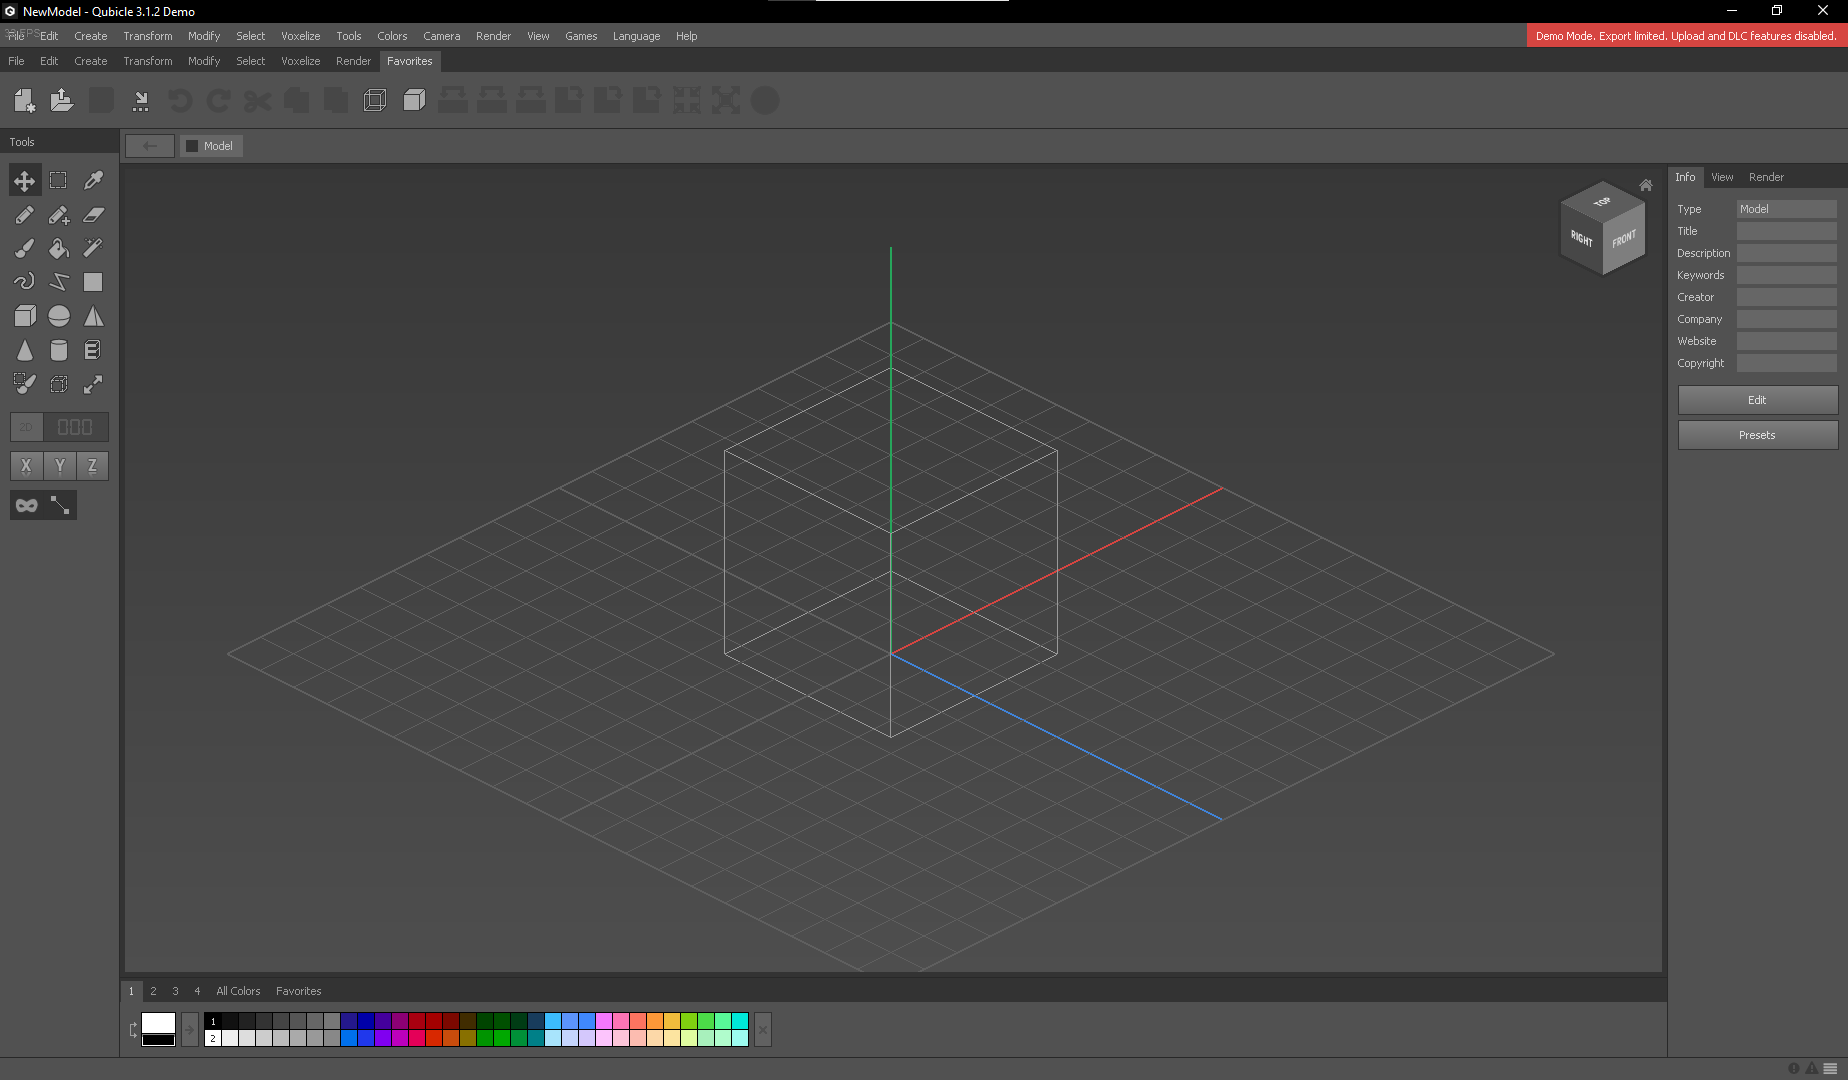
\includegraphics[width=0.9\textwidth, keepaspectratio]{grafika/qubicle.png}
\caption[Ekran startowy programu Qubicle (Windows, Steam)]{Ekran startowy programu Qubicle (Windows, Steam), �r�d�o: \cite{qubicle_page}}
\label{rys1.3-qubicle}
\end{figure}

G��wne atuty oprogramowania wed�ug producenta:
\begin{itemize}
\item Bardzo du�o narz�dzi do edycji.
\item Proste w obs�udze.
\item Wbudowane narz�dzie do konwersji z modelu siatkowego na model wokselowy.
\item Wiele format�w do eksportu modeli.
\end{itemize}

Qubicle jest dost�pny w czterech wersjach na platformach Windows i macOS, wersja okrojona (demo) za darmo, wersja podstawowa (bazowa) za 53.99 PLN, wersja rozszerzona (indie) za 89.99 PLN i pe�na opcja (pro) za 410.56 PLN.

\section{Goxel}

Goxel \cite{goxel_page} jest otwartym oprogramowaniem do edycji modeli wokselowych na komputery osobiste i urz�dzenia mobilne stworzone przez u�ytkownika o pseudonimie @guillaumechereau (GitHub). G��wn� funkcjonalno�ci� Goxel, jest mo�liwo�� tworzenia warstw, w taki sam spos�b jak w popularnych aplikacjach do manipulacji obrazami, mi�dzy innymi takim jaki jest Adobe Photoshop. Interfejs  rozwi�zania zosta� przedstawiony na rysunku \ref{rys1.4-goxel}

\begin{figure}[htb]
\centering
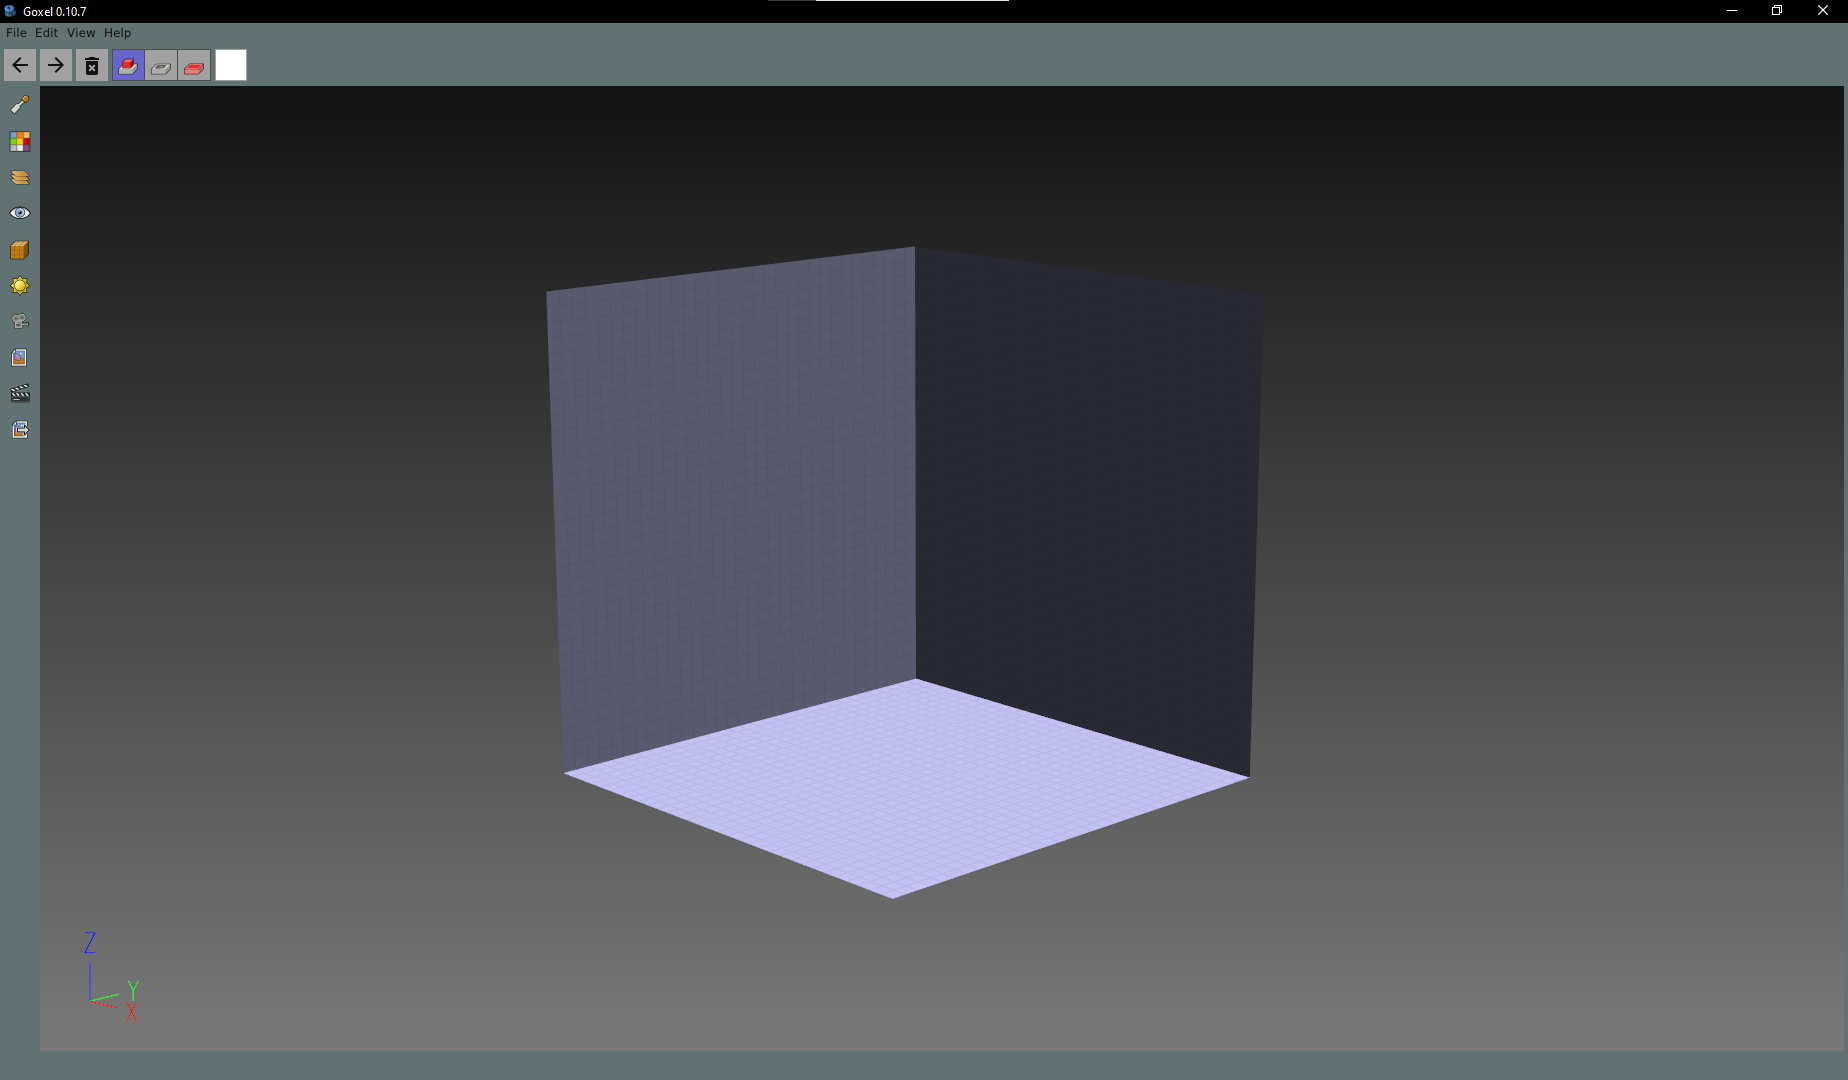
\includegraphics[width=0.9\textwidth, keepaspectratio]{grafika/goxel.png}
\caption[Ekran Startowy programu Goxel (Windows)]{Ekran Startowy programu Goxel (Windows), �r�d�o: \cite{goxel_page}}
\label{rys1.4-goxel}
\end{figure}

G��wne atuty oprogramowania wed�ug producenta:
\begin{itemize}
\item Niesko�czona wielko�� sceny.
\item Mo�liwo�� tworzenia obiekt�w na r�nych warstwach.
\item Wieloplatformowo��.
\item Wiele format�w do eksportu modeli.
\end{itemize}

Goxel jest dost�pny za darmo na platformach Windows, Linux, iOS i macOS, a w przypadku platformy Android za op�at� 25.99 PLN.

\section{VoxEdit Beta}

VoxEdit Beta \cite{voxedit_beta_page} jest darmowym oprogramowaniem stworzonym przez Pixowl do gry The Sandbox Game. Unikaln� funkcjonalno�ci� na tle innych aplikacji do edycji wokseli, jest mo�liwo�� montowania szkieletu i jego p�niejszej animacji. Interfejs  rozwi�zania zosta� przedstawiony na rysunku \ref{rys1.5-voxedit-beta}

\begin{figure}[htb]
\centering
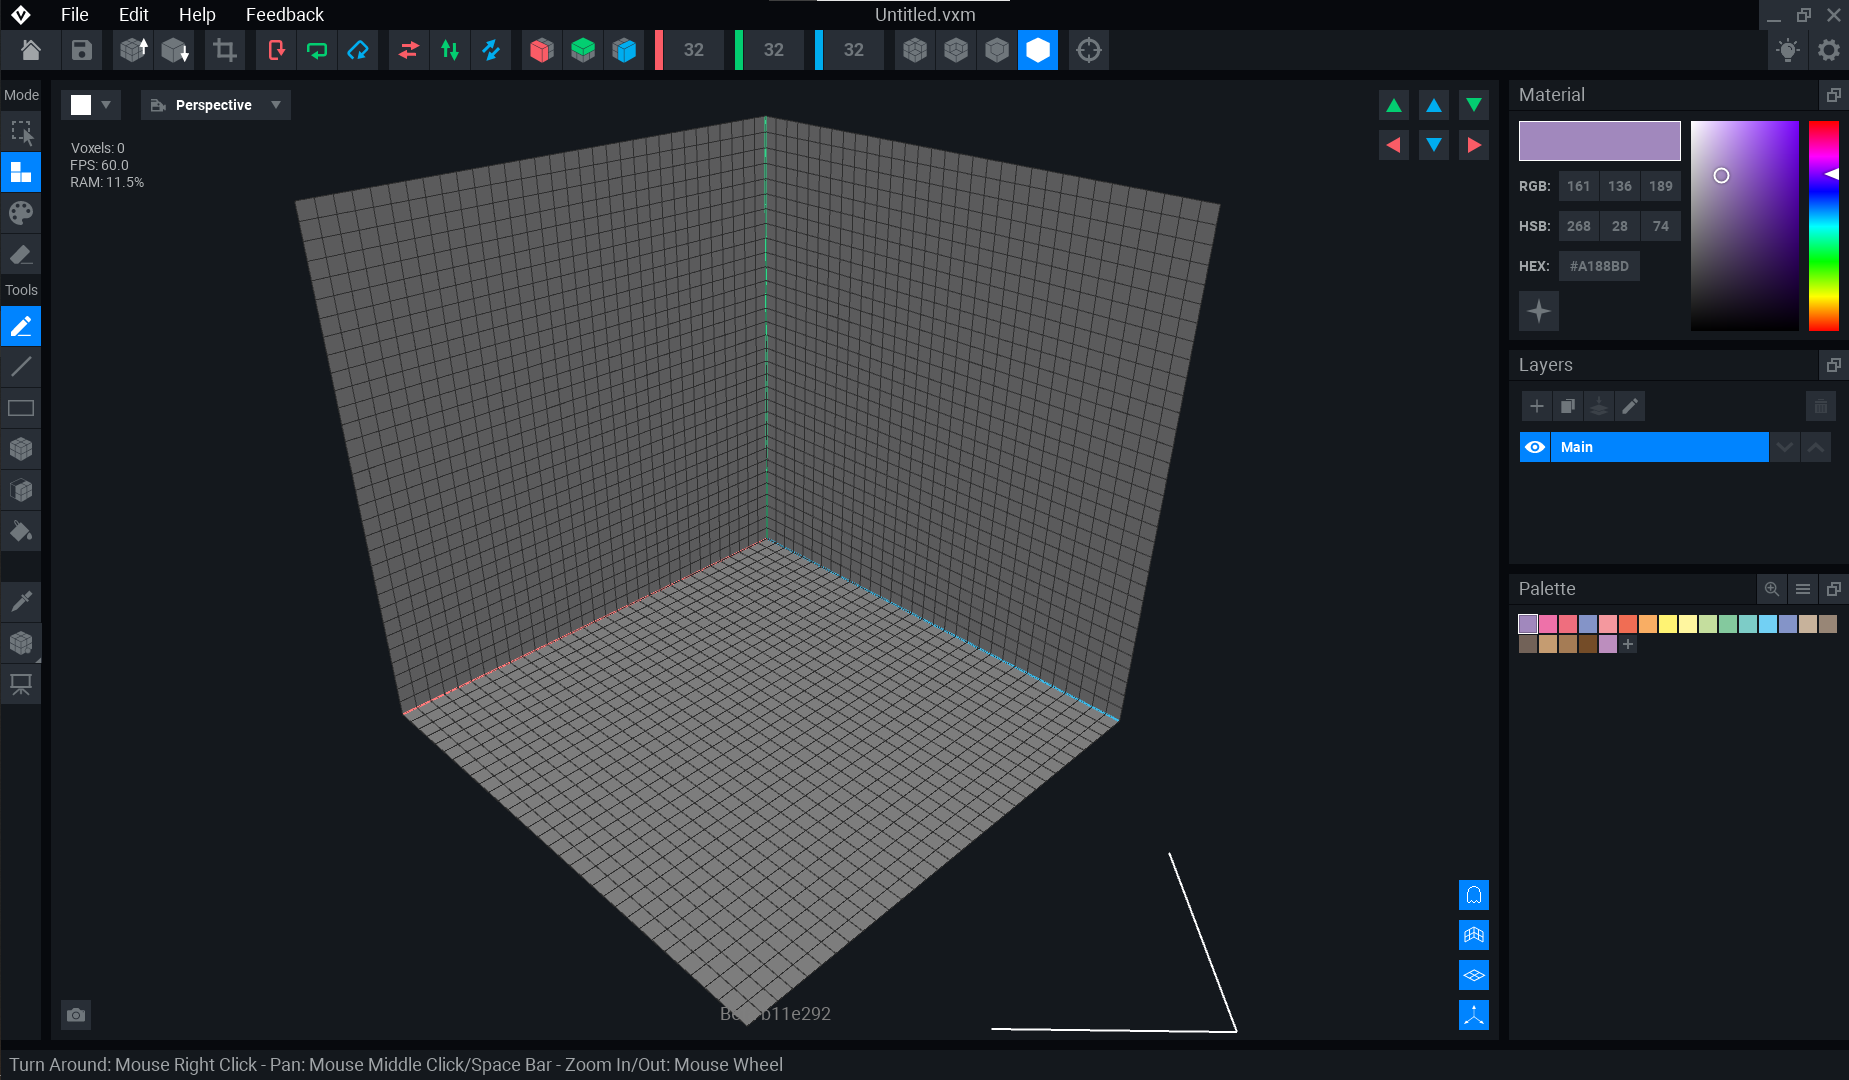
\includegraphics[width=0.9\textwidth, keepaspectratio]{grafika/voxedit-beta.png}
\caption[Ekran startowy programu VoxEdit Beta (Windows)]{Ekran startowy programu VoxEdit Beta (Windows), �r�d�o: \cite{voxedit_beta_page}}
\label{rys1.5-voxedit-beta}
\end{figure}

G��wne atuty oprogramowania wed�ug producenta:
\begin{itemize}
\item Mo�liwo�� tworzenia animacji.
\item Specjalny tryb edycji blok�w.
\item Przyjazny interfejs dla u�ytkownika.
\end{itemize}

VoxEdit Beta jest dost�pny za darmo na platformach Windows i macOS.



\chapter{Projekt systemu}

W tym rozdziale zapoznamy si� z g��wnymi rozwi�zaniami z zakresu in�ynierii oprogramowania i projektowania, kt�re pozwol� nam si� zaznajomi� z podstawowym dzia�aniem aplikacji, jak i wymog�w co do niniejszej pracy.





\section{Wymagania}





Na podstawie informacji zebranych z rozdzia�u 1 ,,Przegl�d istniej�cych rozwi�za�'', jak i mojej wiedzy na temat program�w graficznych, okre�lone zosta�y podstawowe wymagania dotycz�ce aplikacji.

\subsection{Wymagania funkcjonalne}

\begin{itemize}
\item Tworzenie modeli 3D.
\item Prosty interfejs u�ytkownika.
\item Zmiana pozycji i wielko�ci okienek.
\item Edycja modeli w czasie rzeczywistym.
\item Tworzenie w�asnych opis�w materia��w
\item Zapis i odczyt modelu.
\item Zmiana w�a�ciwo�ci o�wietlenia.
\end{itemize}

\subsection{Wymagania niefunkcjonalne}

\begin{itemize}
\item Mo�liwo�� ponownego u�ycia silnika 3D w innych projektach.
\item Wysoka responsywno�� na zmiany w modelu.
\item Dzia�anie na wielu platformach desktopowych (Windows, Linux, macOS).
\item Konsola debuguj�ca w czasie rzeczywistym.
\end{itemize}






\section{Interfejs graficzny}





G��wnym za�o�eniem interfejsu by�a prostota i customizowalno��. Osi�gni�te to zosta�o poprzez wyeksponowanie modelu, kt�ry jest renderowany w czasie rzeczywistym przez silnik 3D edytora. 

\begin{figure}[htb]
\centering
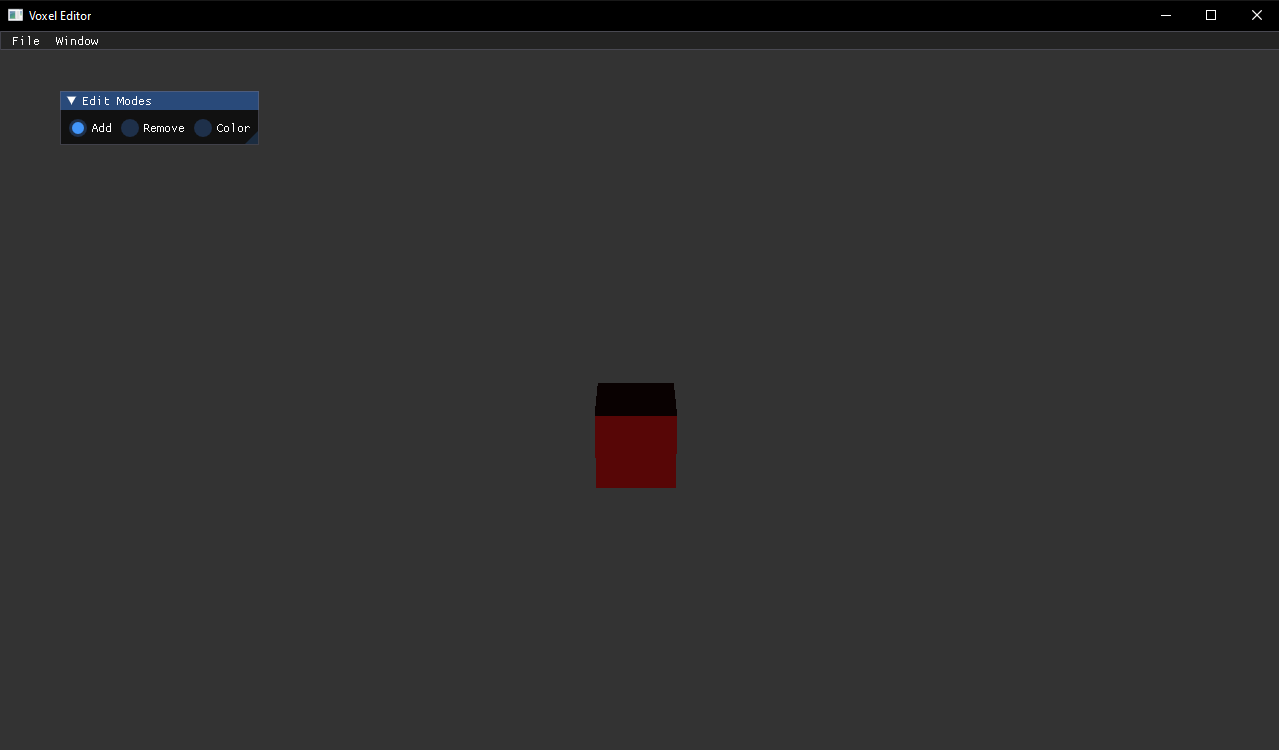
\includegraphics[width=0.9\textwidth, keepaspectratio]{grafika/voxel-editor-main.png}
\caption{Ekran startowy programu, �r�d�o: opracowanie w�asne} 
\label{rys-voxel-editor-main}
\end{figure}

By u�ytkownikowi da� wi�cej mo�liwo�ci ustawienia wygl�du wyj�ciowego, dodano opcj� zmiany warto�ci o�wietlenia, jak i t�a aplikacji. Wygl�d okna ,,Scene'' zosta� ukazany na rysunku \ref{rys-voxel-editor-scene-edit}.

\begin{figure}[htb]
\centering
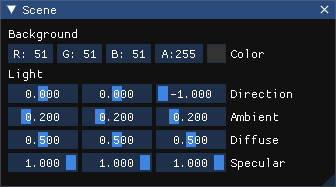
\includegraphics[width=0.6\textwidth, keepaspectratio]{grafika/voxel-editor-scene-edit.png}
\caption{Okno zmiany ustawie� sceny, �r�d�o: opracowanie w�asne} 
\label{rys-voxel-editor-scene-edit}
\end{figure}

Zmiana aktywnego materia�u odbywa si� poprzez wyb�r z listy dost�pnych, jak i stworzonych materia��w w oknie ,,Material'' (rysunek \ref{rys-voxel-editor-material-edit}).

\begin{figure}[htb]
\centering
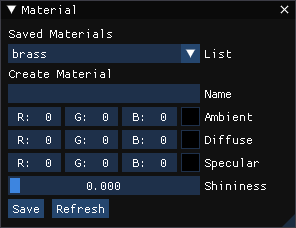
\includegraphics[width=0.6\textwidth, keepaspectratio]{grafika/voxel-editor-material-edit.png}
\caption{Okno zmiany bie��cego materia�u, jak i jego edycji, �r�d�o: opracowanie w�asne} 
\label{rys-voxel-editor-material-edit}
\end{figure}

W celu u�atwienia wyboru koloru podczas tworzenia materia�u oraz wyboru t�a sceny, parametry ,,Color'' w przypadku okna ,,Scene'', jak i ,,Ambient'', ,,Diffuse'' i ,,Specular'' w przypadku okna ,,Material'' posiadaj� opcj� wyboru r�cznego z kwadratu kolor�w (rysunek \ref{rys-voxel-editor-rgb}).

\begin{figure}[htb]
\centering
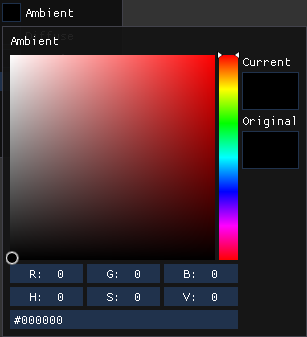
\includegraphics[width=0.5\textwidth, keepaspectratio]{grafika/voxel-editor-rgb.png}
\caption{Okno wyboru warto�ci koloru wraz z podgl�dem po prawej stronie, �r�d�o: opracowanie w�asne} 
\label{rys-voxel-editor-rgb}
\end{figure}





\section{Diagram przypadk�w u�ycia i opisy}





Na przedstawionym poni�ej (rysunek \ref{rys-diagram-przypadkow-uzycia}) diagramie przypadk�w u�ycia, zawarte s� wszystkie najwa�niejsze wymagania funkcjonalne w formie graficznej. 

\begin{figure}[htb]
\centering
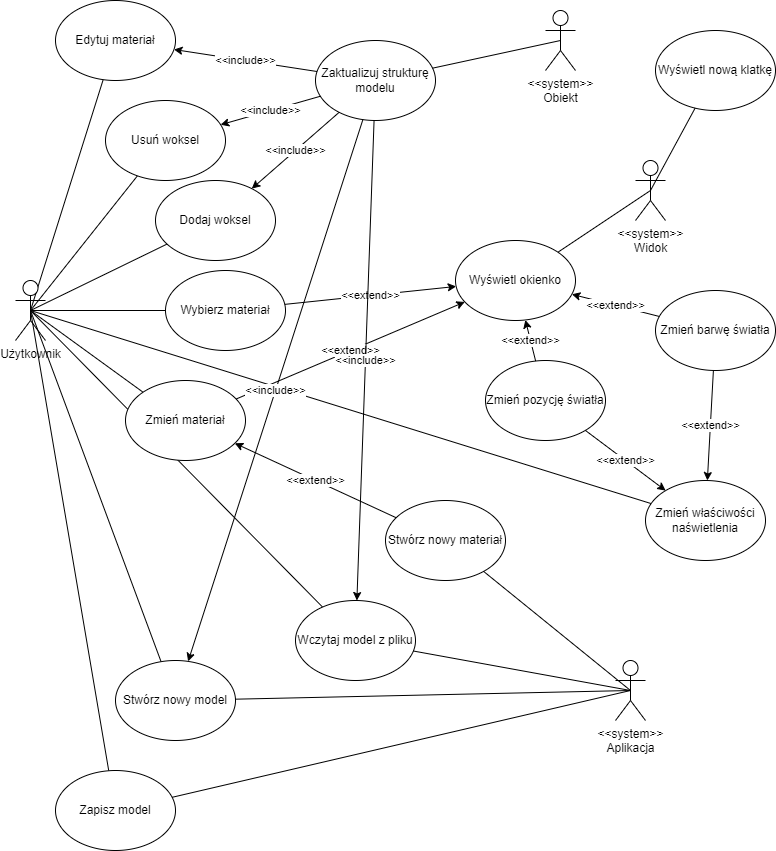
\includegraphics[width=1\textwidth, keepaspectratio]{grafika/diagram-przypadkow-uzycia.png}
\caption{Diagram przypadk�w u�ycia, �r�d�o: opracowanie w�asne} 
\label{rys-diagram-przypadkow-uzycia}
\end{figure}

G��wnymi przypadkami u�ycia tego systemu s� metody manipulacji modelu 3D. To one pozwalaj� nam na dodawanie wokseli, usuwanie ich oraz edytowanie materia�u. Przypadki te s� odpowiednio opisane w tabeli \ref{tabela_dodaj_voksel}, tabeli \ref{tabela_usun_woksel} oraz tabeli \ref{tabela_edytuj_material}.

\begin{table}[htb]
\centering
\caption[Opis przypadku u�ycia ,,Dodaj woksel'']{Opis przypadku u�ycia ,,Dodaj woksel''}
\begin{tabular}{|>{\bfseries}p{.3\textwidth}|p{.7\textwidth}|}
\hline
\rowcolor{Gray}
\rowstyle{\bfseries}
Sekcja & Tre�� \\\hline
Uczestnicz�cy aktorzy & U�ytkownik, Widok, Aplikacja, Obiekt \\\hline
Warunki wst�pne & W okienku ,,Edit Mode'' zaznaczony tryb ,,Add'' \\\hline
Warunki ko�cowe & Dodanie woksela do obiektu \\\hline
Rezultat & Pojawienie si� woksela w miejscu wskazanym przez u�ytkownika \\\hline
Scenariusz g��wny & 
\begin{enumerate}[topsep=0pt, leftmargin=*]
\item U�ytkownik wybiera materia� z listy, b�d� dodaje sw�j w�asny i go
zatwierdza.
\item U�ytkownik nacelowuje na interesuj�c� go sciank� woksela, w celu postawienia na obok niej nowego woksela, po czym zatwierdza prawym przyciskiem myszy.
\item Aplikacja przekazuje do obiektu dane klikni�cia.
\item Obiekt aktualizuje struktur� danych.
\item Widok zostaje od�wie�ony w nast�pnej klatce.
\item U�ytkownik widzi efekt swojego dzia�ania na modelu 3D.
\end{enumerate} \\\hline
Scenariusz wyj�tku & Zdarzenie: U�ytkownik nie klikn�� na �ciank� istniej�cego woksela 

Wynik: Brak dodania woksela do modelu 3D \\\hline
Zale�no�ci czasowe & \begin{enumerate}[topsep=0pt, leftmargin=*]
\item Cz�stotliwo�� wykonania: 0 lub wi�cej na sesj�.
\item Typowy czas realizacji: 8.9 ms.
\item Maksymalny czas realizacji: 33,2 ms. 
\end{enumerate} \\\hline
Warto�ci uzyskane przez aktor�w po zako�czeniu przypadk�w u�ycia & \begin{enumerate}[topsep=0pt, leftmargin=*]
\item Pojawienie si� woksela w miejscu i o materiale wybranym przez u�ytkownika.
\item Obiekt posiada zaktualizowan� struktur� o woksela.
\end{enumerate} \\\hline
\end{tabular}
\label{tabela_dodaj_voksel}
\end{table}

\begin{table}[htb]
\centering
\caption[Opis przypadku u�ycia ,,Usu� woksel'']{Opis przypadku u�ycia ,,Usu� woksel''}
\begin{tabular}{|>{\bfseries}p{.3\textwidth}|p{.7\textwidth}|}
\hline
\rowcolor{Gray}
\rowstyle{\bfseries}
Sekcja & Tre�� \\\hline
Uczestnicz�cy aktorzy & U�ytkownik, Widok, Aplikacja, Obiekt  \\\hline
Warunki wst�pne & W okienku ,,Edit Mode'' zaznaczony tryb ,,Remove''  \\\hline
Warunki ko�cowe & Usuni�cie wskazanego woksela z obiektu \\\hline
Rezultat & Znikni�cie woksela w miejscu wskazanym przez u�ytkownika \\\hline
Scenariusz g��wny & 
\begin{enumerate}[topsep=0pt, leftmargin=*]
\item U�ytkownik nacelowuje na interesuj�cy go woksel, po czym zatwierdza
prawym przyciskiem myszy.
\item Aplikacja przekazuje do obiektu dane klikni�cia.
\item Obiekt zwraca woksel zainteresowania.
\item Aplikacja usuwa zwr�cony woksel.
\item Widok zostaje od�wie�ony w nast�pnej klatce.
\item U�ytkownik widzi efekt swojego dzia�ania na modelu 3D.
\end{enumerate} \\\hline
Scenariusz wyj�tku & Zdarzenie: U�ytkownik nie klikn�� w istniej�cego woksela 

Wynik: Brak usuni�cia woksela z modelu 3D \\\hline
Zale�no�ci czasowe & \begin{enumerate}[topsep=0pt, leftmargin=*]
\item Cz�stotliwo�� wykonania: 0 lub wi�cej na sesj�.
\item Typowy czas realizacji: 5.9 ms.
\item Maksymalny czas realizacji: 16,6 ms. 
\end{enumerate} \\\hline
Warto�ci uzyskane przez aktor�w po zako�czeniu przypadk�w u�ycia & \begin{enumerate}[topsep=0pt, leftmargin=*]
\item Znikni�cie woksela w miejscu wybranym przez u�ytkownika.
\item Obiekt posiada zaktualizowan� struktur� bez klikni�tego woksela.
\end{enumerate} \\\hline
\end{tabular}
\label{tabela_usun_woksel}
\end{table}

\begin{table}[htb]
\centering
\caption[Opis przypadku u�ycia ,,Edytuj materia�'']{Opis przypadku u�ycia ,,Edytuj materia�''}
\begin{tabular}{|>{\bfseries}p{.3\textwidth}|p{.7\textwidth}|}
\hline
\rowcolor{Gray}
\rowstyle{\bfseries}
Sekcja & Tre�� \\\hline
Uczestnicz�cy aktorzy & U�ytkownik, Widok, Aplikacja, Obiekt  \\\hline
Warunki wst�pne & W okienku ,,Edit Mode'' zaznaczony tryb ,,Color''  \\\hline
Warunki ko�cowe & Zmiana materia�u we wskazanym miejscu w obiekcie \\\hline
Rezultat & Zmiana materia�u woksela w miejscu wskazanym przez u�ytkownika \\\hline
Scenariusz g��wny & 
\begin{enumerate}[topsep=0pt, leftmargin=*]
\item U�ytkownik nacelowuje na interesuj�cy go woksel, po czym zatwierdza
prawym przyciskiem myszy.
\item Aplikacja przekazuje do obiektu dane klikni�cia.
\item Obiekt zwraca woksel zainteresowania.
\item Aplikacja zmiania kolor zwr�conego woksela na ostatni wybrany materia�.
\item Widok zostaje od�wie�ony w nast�pnej klatce.
\item U�ytkownik widzi efekt swojego dzia�ania na modelu 3D.
\end{enumerate} \\\hline
Scenariusz wyj�tku & Zdarzenie: U�ytkownik nie klikn�� w istniej�cego woksela 

Wynik: Brak zmiany koloru woksela w modelu 3D \\\hline
Zale�no�ci czasowe & \begin{enumerate}[topsep=0pt, leftmargin=*]
\item Cz�stotliwo�� wykonania: 0 lub wi�cej na sesj�.
\item Typowy czas realizacji: 3.2 ms.
\item Maksymalny czas realizacji: 16,6 ms. 
\end{enumerate} \\\hline
Warto�ci uzyskane przez aktor�w po zako�czeniu przypadk�w u�ycia & \begin{enumerate}[topsep=0pt, leftmargin=*]
\item Zmiana w�a�ciwo�ci materia�u woksela w miejscu wybranym przez u�ytkownika.
\item Obiekt posiada zmienion� specyfikacje materia�u w klikni�tym wokselu.
\end{enumerate} \\\hline
\end{tabular}
\label{tabela_edytuj_material}
\end{table}




\section{Diagramy stan�w}




\begin{figure}[htb]
\centering
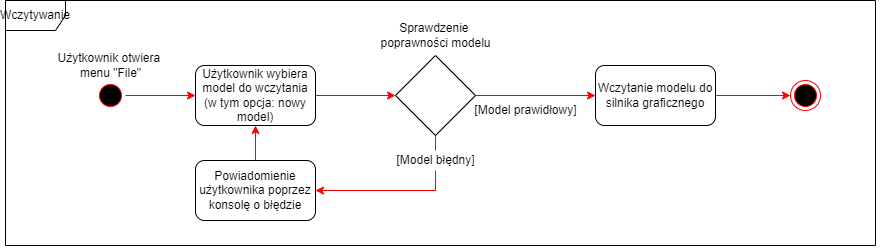
\includegraphics[width=0.9\textwidth, keepaspectratio]{grafika/diagram-stanow-wczytywanie.png}
\caption{Diagram stan�w dla wczytywania, �r�d�o: opracowanie w�asne} 
\label{rys-diagram-stanow-wczytywanie}
\end{figure}

\begin{figure}[htb]
\centering
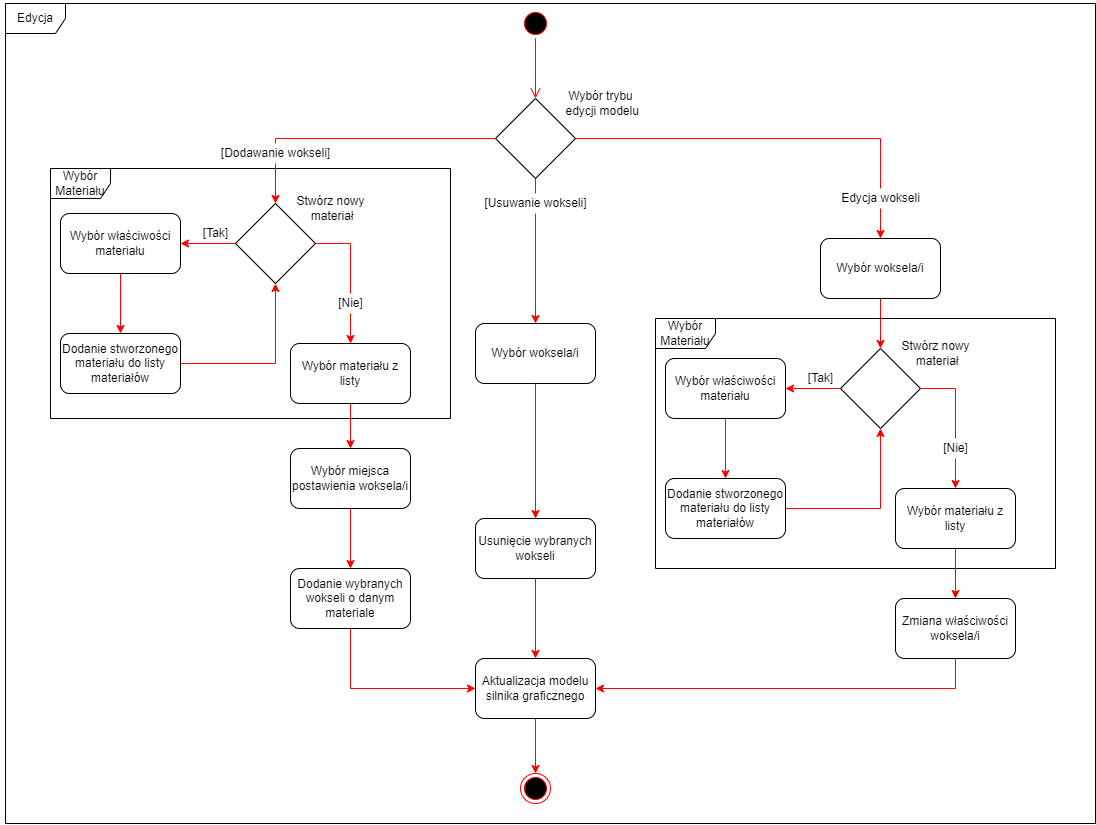
\includegraphics[width=0.9\textwidth, keepaspectratio]{grafika/diagram-stanow-edycja.png}
\caption{Diagram stan�w dla edycji, �r�d�o: opracowanie w�asne} 
\label{rys-diagram-stanow-edycja}
\end{figure}



\chapter{Rozdzia� 3}

Prosta tabela \ref{tabela_1}.

\begin{table}[htb]
\centering
\caption[Kr�tki podpis tabeli 1 -- do spisu tre�ci]{D�ugi podpis tabeli 1, kt�ry pojawi si� nad ni�. Jak chcecie podpis pod tabel�, umie��cie caption przed samym end\{table\} - ale to niezgodne z wytycznymi.}
\begin{tabular}{|c|c|c|c|}
\hline
Kolumna 1 & Kolumna 2 & Kolumna 3 & Kolumna 4 \\\hline
Kolumna 1 & Kolumna 2 & Kolumna 3 & Kolumna 4 \\\hline
Kolumna 1 & Kolumna 2 & Kolumna 3 & Kolumna 4 \\\hline
Kolumna 1 & Kolumna 2 & Kolumna 3 & Kolumna 4 \\\hline
\end{tabular}
\label{tabela_1}
\end{table}

Przyk�adowa tabela \ref{tabela_2}, nieco bardziej skomplikowana.

\begin{table}[htb]
\centering
\caption[Kr�tki podpis tabeli 2 -- do spisu tre�ci]{D�ugi podpis tabeli 2, kt�ry pojawi si� nad ni�}
\scalebox{0.6}{
\begin{tabular}{|>{\bfseries}!a||^c|^c|^c|^c|^c|^c|^c|^c|^c|^c|}
\hline
\rowcolor{Gray}
\rowstyle{\bfseries}
Kolumna wyr�niona & \makecell{Kolumna \\ pierwsza} & \makecell{Kolumna \\ druga}& \makecell{Kolumna \\ kolejna \\ d�uga \\ nazwa} & \makecell{Przeno- \\ szenie \\ s�owa} & \makecell{Kolumna \\ kolejna} & \makecell{Kolumna \\ kolejna} & \makecell{Kolumna \\ kolejna} & \makecell{Kolumna \\ kolejna} & \makecell{Kolumna \\ kolejna} & \makecell{Kolumna \\ kolejna} \\\hline
Wiersz jaki� tam & 1 & 2 & \cellcolor{LightGray}3 & 4 & 5 & 6 & 7 & \cellcolor{LightGray}8 & 9 & 10 \\\hline \hline
Wiersz ze statystykami & 11,56 & 92,38 & 827,21 & 41,92 & 29,71 & 28,77 & \cellcolor{LightRed}29,61 & 55,02 & 72,33 & 95,82 \\\hline
Wiersz ze statystykami & 11,56 & \textbf{92,38} & 827,21 & 41,92 & 29,71 & \cellcolor{LightGreen}28,77 & 29,61 & 55,02 & 72,33 & \cellcolor{LightRed}95,82 \\\hline
Wiersz ze statystykami & 11,56 & \textbf{92,38} & 827,21 & 41,92 & 29,71 & 28,77 & 29,61 & 55,02 & \cellcolor{LightGreen}72,33 & 95,82 \\\hline
Wiersz ze statystykami & 11,56 & 92,38 & \cellcolor{LightGreen}827,21 & 41,92 & 29,71 & 28,77 & 29,61 & 55,02 & 72,33 & 95,82 \\\hline
Wiersz ze statystykami & \cellcolor{LightGreen}11,56 & 92,38 & \cellcolor{LightRed}827,21 & 41,92 & 29,71 & 28,77 & 29,61 & 55,02 & 72,33 & 95,82 \\\hline
Wiersz ze statystykami & 11,56 & 92,38 & 827,21 & \textbf{41,92} & 29,71 & 28,77 & 29,61 & 55,02 & \cellcolor{LightRed}72,33 & 95,82 \\\hline
Wiersz ze statystykami & 11,56 & 92,38 & 827,21 & 41,92 & 29,71 & 28,77 & \cellcolor{LightRed}29,61 & 55,02 & 72,33 & 95,82 \\\hline
Wiersz ze statystykami & 11,56 & \cellcolor{LightGreen}92,38 & 827,21 & 41,92 & 29,71 & 28,77 & \cellcolor{LightGreen}29,61 & 55,02 & 72,33 & 95,82 \\\hline
Wiersz ze statystykami & 11,56 & \cellcolor{LightRed}92,38 & 827,21 & 41,92 & 29,71 & 28,77 & \textbf{29,61} & 55,02 & 72,33 & 95,82 \\\hline
Wiersz ze statystykami & 11,56 & 92,38 & 827,21 & 41,92 & \cellcolor{LightRed}29,71 & \cellcolor{LightRed}28,77 & 29,61 & 55,02 & 72,33 & 95,82 \\\hline \hline
\end{tabular}
}
\label{tabela_2}
\end{table}
\chapter{Rozdzia� 4}


\chapter{Dokumentacja techniczna}

Dokumentacja techniczna aplikacji stanowi wa�ny element u�ytkownika do nawigacji po systemie. Zapewnia ona wprowadzenie do wygl�du aplikacji, jak i opisuje w jaki spos�b osi�gn�� po��dany efekt w aplikacji.

\section{Prezentacja systemu}

G��wnym za�o�eniem interfejsu by�a prostota i customizowalno��. Osi�gni�te to zosta�o poprzez wyeksponowanie modelu, kt�ry jest renderowany w czasie rzeczywistym przez silnik 3D edytora. 

\begin{figure}[htb]
\centering
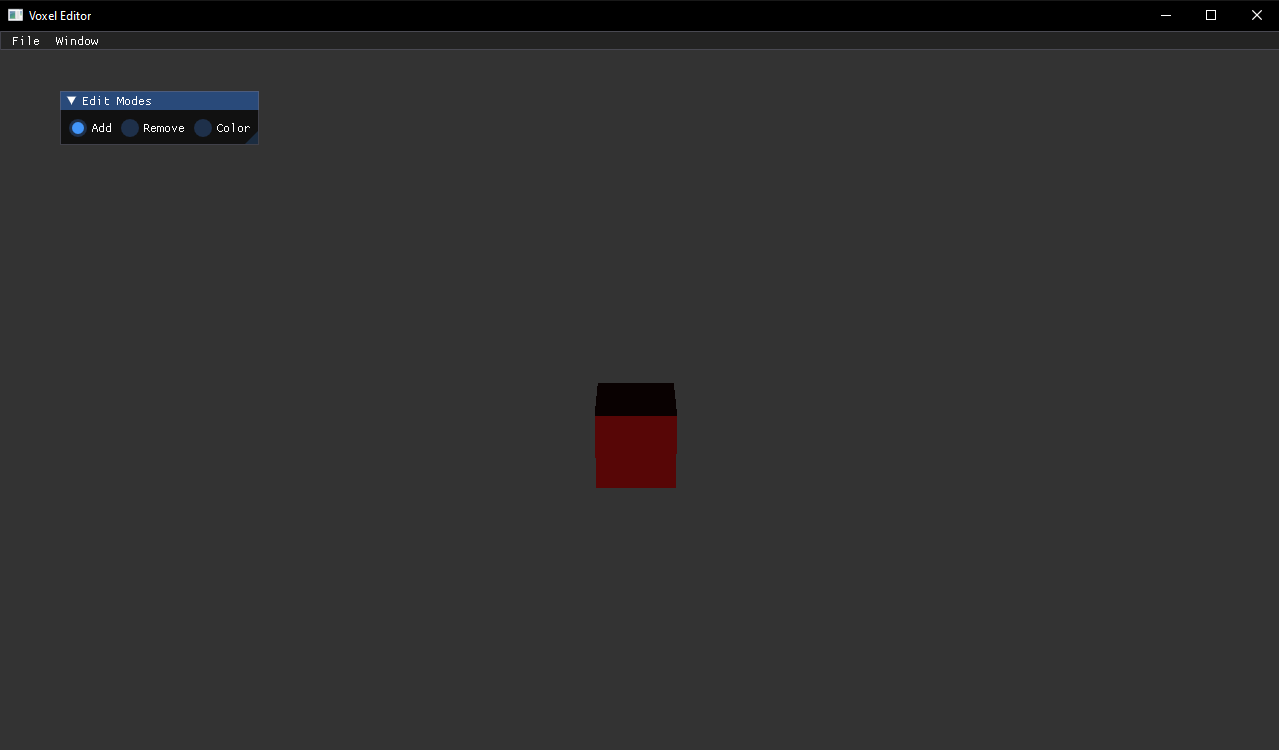
\includegraphics[width=0.9\textwidth, keepaspectratio]{grafika/voxel-editor-main.png}
\caption{Ekran startowy programu, �r�d�o: opracowanie w�asne} 
\label{rys-voxel-editor-main}
\end{figure}

\subsection{Okno ,,Scene''}

By u�ytkownikowi da� wi�cej mo�liwo�ci ustawienia wygl�du wyj�ciowego, dodano opcj� zmiany warto�ci o�wietlenia, jak i t�a aplikacji. Wygl�d okna ,,Scene'' zosta� ukazany na rysunku \ref{rys-voxel-editor-scene-edit}.

\begin{figure}[htb]
\centering
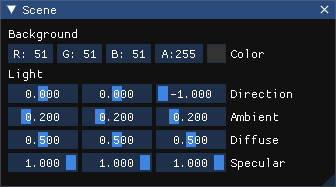
\includegraphics[width=0.6\textwidth, keepaspectratio]{grafika/voxel-editor-scene-edit.png}
\caption{Okno zmiany ustawie� sceny, �r�d�o: opracowanie w�asne} 
\label{rys-voxel-editor-scene-edit}
\end{figure}

\subsection{Okno ,,Material''}

Zmiana aktywnego materia�u odbywa si� poprzez wyb�r z listy dost�pnych, jak i stworzonych materia��w w oknie ,,Material'' (rysunek \ref{rys-voxel-editor-material-edit}).

\begin{figure}[htb]
\centering
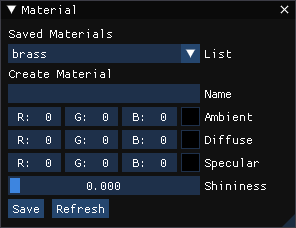
\includegraphics[width=0.6\textwidth, keepaspectratio]{grafika/voxel-editor-material-edit.png}
\caption{Okno zmiany bie��cego materia�u, jak i jego edycji, �r�d�o: opracowanie w�asne} 
\label{rys-voxel-editor-material-edit}
\end{figure}

\subsection{Podgl�d wybranego koloru}

W celu u�atwienia wyboru koloru podczas tworzenia materia�u oraz wyboru t�a sceny, parametry ,,Color'' w przypadku okna ,,Scene'', jak i ,,Ambient'', ,,Diffuse'' i ,,Specular'' w przypadku okna ,,Material'' posiadaj� opcj� wyboru r�cznego z kwadratu kolor�w (rysunek \ref{rys-voxel-editor-rgb}).

\begin{figure}[htb]
\centering
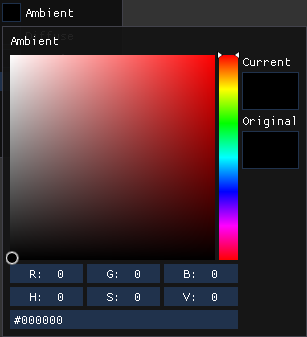
\includegraphics[width=0.5\textwidth, keepaspectratio]{grafika/voxel-editor-rgb.png}
\caption{Okno wyboru warto�ci koloru wraz z podgl�dem po prawej stronie, �r�d�o: opracowanie w�asne} 
\label{rys-voxel-editor-rgb}
\end{figure}

\subsection{Okno ,,Debug''}

Okno ,,Debug'' (rysunek \ref{rys-voxel-editor-debug-edit}) powsta�o specjalnie z uwag� na wymagania czasowe dotycz�ce g��wnych funkcjonalno�ci. Przycisk ,,WireFrame mode'' prze��cza w silniku 3D spos�b renderowania obiekt�w na tylko kraw�dzie, za� przycisk ,,Optimized mode'' pozwala na wy��czenie zoptymalizowanego algorytmu rysowania modelu. Pod przyciskami w czasie rzeczywistym kre�lony jest wykres czasu renderowania pojedynczej klatki (ang. \textit{frame time}).

\begin{figure}[htb]
\centering
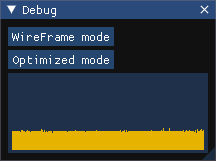
\includegraphics[width=0.4\textwidth, keepaspectratio]{grafika/voxel-editor-debug-edit.png}
\caption{Okno z informacjami o dzia�aniu silnika graficznego, �r�d�o: opracowanie w�asne} 
\label{rys-voxel-editor-debug-edit}
\end{figure}

\subsection{Zarz�dzanie oknami}

Przedstawione powy�ej okna aplikacji, s� dost�pne z poziomu paska nawigacji (rysunek \ref{rys-voxel-editor-window-options}) za pomoc� kt�rego mo�na je pokazywa� lub chowa�. Dla ka�dego z tych okienek, u�ytkownik mo�e zmieni� ich pozycj�, wielko��, jak i zminimalizowa�, wed�ug w�asnego uznania. Na rysunku \ref{rys-voxel-editor-small} przedstawione zosta�o zmniejszone okno ,,Material'' z rysunku \ref{rys-voxel-editor-material-edit}. 

\begin{figure}[htb]
\centering
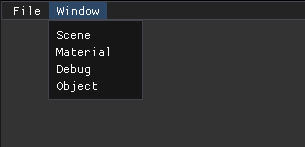
\includegraphics[width=0.5\textwidth, keepaspectratio]{grafika/voxel-editor-window-options.png}
\caption{Pasek nawigacyjny z wybran� opcj� ,,Window'', �r�d�o: opracowanie w�asne} 
\label{rys-voxel-editor-window-options}
\end{figure}

\begin{figure}[htb]
\centering
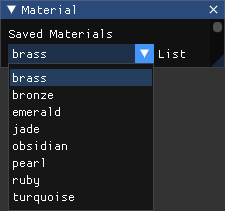
\includegraphics[width=0.4\textwidth, keepaspectratio]{grafika/voxel-editor-small.png}
\caption{Okno ,,Material'' ze zmienionym rozmiarem przez u�ytkownika, �r�d�o: opracowanie w�asne} 
\label{rys-voxel-editor-small}
\end{figure}

\subsection{Okno ,,Edit Modes''}

G��wnym oknem do zmiany tryb�w interakcji z modelem 3D jest ,,Edit Modes'' ukazany na rysunku \ref{rys-voxel-editor-edit-mode}. S�u�y ono do zmiany g��wnych tryb�w edycji na modelu 3D. Przez zaznaczenie jednej opcji z ,,Add'', ,,Remove'' lub ,,Color'', klikni�cie na istniej�cy model na ekranie b�dzie mia� inny rezultat.

\begin{figure}[htb]
\centering
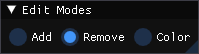
\includegraphics[width=0.4\textwidth, keepaspectratio]{grafika/voxel-editor-edit-mode.png}
\caption{Okno trybu edycji modelu 3D, �r�d�o: opracowanie w�asne} 
\label{rys-voxel-editor-edit-mode}
\end{figure}

\subsection{Okna manipulacji plikami}

Pasek z rysunku \ref{rys-voxel-editor-window-options} posiada jeszcze jedn� opcj�, a mianowicie ,,File'', odpowiedzialn� za wczytywanie modeli z pliku, zapisywanie ich oraz tworzenie nowych. Opcj� tej zak�adki s� przedstawione na rysunku \ref{rys-voxel-editor-file-options}

\begin{figure}[htb]
\centering
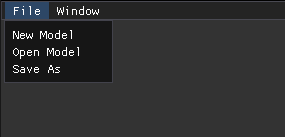
\includegraphics[width=0.4\textwidth, keepaspectratio]{grafika/voxel-editor-file-options.png}
\caption{Pasek nawigacyjny z wybran� opcj� ,,File'', �r�d�o: opracowanie w�asne} 
\label{rys-voxel-editor-file-options}
\end{figure}

W przypadku opcji ,,Open Model'' przedstawionej na rysunku \ref{rys-voxel-editor-open} oraz ,,Save As'' na rysunku \ref{rys-voxel-editor-save-as}, u�ytkownik wprowadza �cie�k� wzgl�dn� do pliku w celu jego wczytania, b�d� w przypadku opcji drugiej, jego nazw�. 

\begin{figure}[htb]
\centering
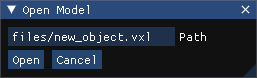
\includegraphics[width=0.4\textwidth, keepaspectratio]{grafika/voxel-editor-open.png}
\caption{Okno wczytania modeli do edytora, �r�d�o: opracowanie w�asne} 
\label{rys-voxel-editor-open}
\end{figure}

\begin{figure}[htb]
\centering
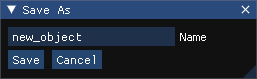
\includegraphics[width=0.4\textwidth, keepaspectratio]{grafika/voxel-editor-save-as.png}
\caption{Okno zapisu aktualnego modelu 3D do pliku, �r�d�o: opracowanie w�asne} 
\label{rys-voxel-editor-save-as}
\end{figure}



\section{Instrukcja u�ytkownika}

W podrozdziale

\chapter{Rozdzia� 6}

\chapter*{Podsumowanie}
\addcontentsline{toc}{chapter}{Podsumowanie}

Tematem niniejszej pracy by�o stworzenie aplikacji pozwalaj�cej na kreacj� modeli 3D opartych o woksele. Cz�� teoretyczna opiera�a si� na zapoznaniu z podstawowymi funkcjonalno�ciami istniej�cych ju� rozwi�za�, jak i dzia�aniem tych aplikacji graficznych, na podstawie kt�rych powsta� projektu systemu. 

W ramach pracy powsta� prosty silnik 3D posiadaj�cy podstawowe funkcjonalno�ci potrzebne do edycji model�w 3D, takie jak dodawanie nowych obiekt�w, usuwanie ich, oraz zmiana ich w�a�ciwo�ci. Dost�p do tych funkcjonalno�ci odbywa si� poprzez interfejs okienkowy,  pe�ni�cy role narz�dzia do edycji modelu. W ten spos�b powsta�a aplikacja pozwoli�a na osi�gni�cie w pe�ni celu niniejszej pracy, kt�rym by�o stworzenie edytora modeli 3D opartych o woksele.

Wykonanie niniejszej pracy pozwoli�o wyci�gn�� szereg wniosk�w. Analiza istniej�cych rozwi�za� na rynku w znaczny spos�b u�atwi�a okre�lenie wymaga� stawionych w projekcie systemu. Zaprojektowanie rozwi�zania przed rozpocz�ciem implementacji u�atwi�o p�niejszy proces tworzenia aplikacji, potwierdzaj�c istot� przygotowania projektu systemu. Dokumentacja techniczna pozwoli�a osobom odpowiedzialnym za testowanie na �atw� konfiguracj� i nawigacj� po oprogramowaniu.

Mimo, �e aplikacja pozwala na tworzenie i edycj� modeli 3D, spe�niaj�c jednocze�nie cel pracy, nie mo�na wykluczy� dalszego rozwoju tego rozwi�zania. Z uwagi na u�ycie silnika graficznego, mo�liwe jest ponowne wykorzystanie silnika w celu stworzenia gry komputerowej. Pozwoli to na jednoczesne posiadanie narz�dzia do tworzenia modeli, operuj�ce na tym samym silniku graficznym, co gra komputerowa, pozwalaj�c na �atwe  tworzenie obiekt�w kompatybilnych z gr�. Mo�liwe jest te� rozszerzenie funkcjonalno�ci samego edytora, dodaj�c po��dane rozwi�zania takie jak mo�liwo�� cofni�cia lub przywr�cenia ostatniej czynno�ci, czy mo�liwo�� wyeksportowania wi�kszej ilo�ci parametr�w silnika graficznego.





\nocite{*}
\bibliographystyle{plain}
\bibliography{bibliografia}
\addcontentsline{toc}{chapter}{Bibliografia}

% \listoffigures
{%
    \let\oldnumberline\numberline%
    \renewcommand{\numberline}{\tablename~\oldnumberline}%
    \listoftables
}
\addcontentsline{toc}{chapter}{Spis tabel}
% \listoffigures
{
    \let\oldnumberline\numberline%
    \renewcommand{\numberline}{\figurename~\oldnumberline}%
    \listoffigures
}
\addcontentsline{toc}{chapter}{Spis rysunk�w}
\lstlistoflistings
\addcontentsline{toc}{chapter}{Spis listing�w}
\raggedbottom
\listofalgorithms
\addcontentsline{toc}{chapter}{Spis algorytm�w}

\end{document}
